\underline{\textbf{Третья глава}} посвящена исследованию эволюции кривых фазового синхронизма (КФС) при фотоиндуцированной ГВГ в германосиликатном ОВ в процессе оптического полинга в режиме самозатравки, где затравочное излучение второй гармоники отсутствует.
%Экспериментальные результаты сопоставлены с численным моделированием на основе модели Б. Антонюка и В. Антонюка, адаптированной с учётом керровского эффекта.

В качестве исследуемого образца выбрано германосиликатное одномодовое на длине волны накачки 1030 нм оптическое волокно FUD-3562. Схема экспериментальной установки представлена на рис.~\cref{fig:synopsis_shg_scheme}. Источником накачки служил импульсный иттербиевый волоконный лазер с перестраиваемой длиной волны в диапазоне 1031.9--1032.6 нм, пиковой мощностью до 4 кВт, длительностью импульсов 2 нс и частотой повторения 5 МГц. Исследуемое ОВ длиной 1 м помещалось в термостат для контроля температуры с точностью 0.1°C. Для разделения излучения накачки и второй гармоники использовался набор дихроичных зеркал. Предварительно было установлено, что при мощности накачки до 500 Вт свойства $\chi^{(2)}$-решётки остаются неизменными, поэтому измерение кривых фазового синхронизма проводилось при мощности 50 Вт.

\begin{figure}[h]
	\centering
	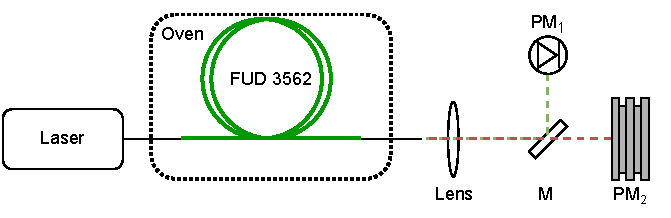
\includegraphics[width=0.8\linewidth]{Dissertation/images/fibershg/scheme}
	\caption{Схема экспериментальной установки}
	\label{fig:synopsis_shg_scheme}
\end{figure}

Методика эксперимента заключалась в следующем. Температура ОВ и длина волны накачки устанавливались равными 22°C и 1032.42 нм соответственно. Излучение накачки пиковой мощностью 4 кВт пропускалось через ОВ для записи $\chi^{(2)}$-решётки. В процессе облучения контролировалась мощность второй гармоники, и после достижения определённого уровня запускалась процедура измерения кривых фазового синхронизма: мощность накачки уменьшалась до 50~Вт, после чего измерялась спектральная кривая синхронизма (перестройкой длины волны накачки) и температурная кривая (изменением температуры ОВ). Затем параметры возвращались к исходным для продолжения записи решётки. Процедура повторялась до достижения стационарного уровня мощности второй гармоники.

Для проверки воспроизводимости эксперимент проведён на двух образцах; результаты идентичны. Контрольные измерения подтвердили, что $\chi^{(2)}$-решётка формируется только в германосиликатном волокне, а её релаксация в течение месяца не наблюдалась.